\documentclass{article}
\usepackage{graphicx}
\usepackage[spanish]{babel}
\usepackage{fancyhdr}
\usepackage{hyperref}
\usepackage{changepage}
\usepackage{setspace}
\usepackage{caption}
\usepackage{float}
\usepackage{array} %....,,,
\usepackage[table,xcdraw]{xcolor}
\usepackage{xcolor}
\definecolor{mirojo}{RGB}{139,0,0}
\usepackage{geometry}
\geometry{letterpaper,
    left=2.5cm,         % Márgen izquierdo
    right=2.5cm,        % Márgen derecho
    top=2.5cm,          % Márgen superior
    bottom=2.5cm        % Márgen inferior
    }

\title{Proyecto}
\author{Levanx}
\date{\today}

\pagestyle{fancy}
\fancyhf{}
\renewcommand{\headrulewidth}{1pt}
\renewcommand{\headrule}{\hbox to\headwidth{\color{mirojo}\leaders\hrule height \headrulewidth\hfill}}
\rhead[R]{\vspace{0cm}\textit{\footnotesize Informe de proyecto - Innovación y Transformación Digital}}
%--------------------
\fancyfoot{}
\fancyfoot[R]{\rule{\textwidth}{0.4pt}\\ \thepage}

\begin{document}
\begin{doublespace}
\begin{center}
    \vspace*{1cm}

    \centering
    \includegraphics[width=8cm]{img/LogoUTP.png}\\[1cm]
    
    \large{\textbf{Innovación y Transformación Digital}} 
    \\[0.5cm] 
    
    \large{\bf AVANCE DE PROYECTO 1}
    \\[0.5cm] 
    \LARGE \textbf{{Chifa Fu}}
\end{center}
\vspace{2cm}
\large{\bf Docente: }
\begin{center}
    \large{Anselmo Aniceto Valenzuela Zegarra}
\end{center}
\large{\bf Grupo: }
\begin{center}
    \large{Nombre: Cueva Zavaleta Geanny Jacinta\textsuperscript{1}, Lima Lopez Edu Orlando Abel\textsuperscript{2}, Muñoz Manosalva Jhoan Aronith\textsuperscript{3}, Ortiz Florentini Brenda Nicole\textsuperscript{4}, Sullón Lévano Leonardo José\textsuperscript{5}, Virhuez Zavaleta Giovanni Elber\textsuperscript{6}}
\end{center}
\begin{center}
    \large{ Universidad Tecnológica del Perú – Sede: Lima Norte.}
\end{center}
    
\begin{center}
    \large{Código: U22211461, U22242277, U22212625, U22220115, U22202313,U22215913}
\end{center}
\begin{center}
Lima, \today
\end{center}
\newpage
\vspace*{0.1cm}
\tableofcontents
\newpage
\vspace*{0.2cm}
\section{Aspectos Generales}
    \subsection{Presentación de la empresa}
    \noindent Wok \& Roll es un chifa con varias sedes en la ciudad, especializado en ofrecer
platos de cocina china de alta calidad. Con una amplia variedad de opciones y un servicio excepcional, ha logrado ganar la preferencia de los clientes, pero aún depende de ventas exclusivamente presenciales. La empresa busca mejorar su competitividad y ofrecer un servicio más accesible mediante la implementación de una plataforma digital para todos sus clientes.

    \subsection{Problemática}
    \noindent Wok \& Roll es un chifa con varias sedes en la ciudad, especializado en ofrecer
platos de cocina china de alta calidad. Con una amplia variedad de opciones y un servicio excepcional, ha logrado ganar la preferencia de los clientes, pero aún depende de ventas exclusivamente presenciales. La empresa busca mejorar su competitividad y ofrecer un servicio más accesible mediante la implementación de una plataforma digital para todos sus clientes.

    \\
    \subsection{Problema General}
    \noindent ¿Cómo pueden los clientes de Wok \& Roll realizar pedidos en línea de manera fácil, rápida y segura, y cómo puede la empresa gestionar eficientemente estos pedidos y clientes en línea?
    \\
    
    \subsection{Problemas Específicos}
    \begin{itemize}
        \item ¿Cómo diseñar un proceso que permita a los clientes realizar pedidos en línea de forma sencilla e intuitiva?
        \item ¿Cómo garantizar la seguridad en los pedidos en línea y minimizar posibles errores durante el proceso?
        \item ¿Cómo garantizar la seguridad en los pedidos en línea y minimizar posibles errores durante el proceso?
    \end{itemize}

    \section{Objectivos}
    \subsection{Objetivo General}
    \begin{itemize}
        \item Desarrollar un sistema web que permita a los clientes de Wok \& Roll realizar pedidos en línea de forma sencilla, rápida y segura, y que facilite a la empresa la gestión eficiente de dichos pedidos y de los clientes que la realizan.
    \end{itemize}
    \subsection{Objetivos específicos}
    \begin{itemize}
        \item Diseñar una interfaz web intuitiva que permita a los clientes realizar pedidos en línea de manera clara y accesible, sin complicaciones.
        \item Implementar mecanismos de validación y control que garanticen la seguridad y precisión de los pedidos realizados en línea.
        \item Desarrollar un módulo de gestión de administrador que permita a la empresa administrar los pedidos y clientes.
    \end{itemize}
    \newpage
    \vspace*{0.5cm}
    \section{Alcances}
    \begin{itemize}
        \item Área pública: dirigida al cliente, incluye visualización del menú, promociones, y formulario de pedidos.
        \item Área privada (admin): acceso restringido para el personal autorizado. Incluye módulos de seguimiento pedidos, clientes, administradores y manejo del contenido que se visualiza en la página.
    \end{itemize}

    \section{Alternativas de solución}
    \subsection{Alternativa 1: Desarrollo de un Software Web de Gestión de Ventas e Inventario}

    \noindent Es la solución central que permite a los clientes realizar pedidos de manera ordenada, registrarlos en un sistema y gestionarlos desde la cocina hasta la entrega. Incluye funciones básicas como registrar pedidos, asignarlos a mesas o delivery, verificar tiempos de preparación y estado de entrega.\\
    \textbf{Ventajas:}\\
    - Centraliza toda la información de pedidos en una sola plataforma.\\
    - Reduce errores al tomar pedidos manualmente.\\
    - Facilita la comunicación entre meseros, cocina y repartidores.\\
    - Mejora la experiencia del cliente al recibir un servicio más rápido y preciso.\\
    \textbf{Desventajas:}\\
    - Requiere capacitación del personal para usarlo correctamente.\\
    - Si el sistema falla, el restaurante puede quedar sin control temporal de pedidos.\\
    - Costo inicial de implementación y mantenimiento.\\

    \begin{figure}[H]
        \centering
        \vspace*{1cm}
        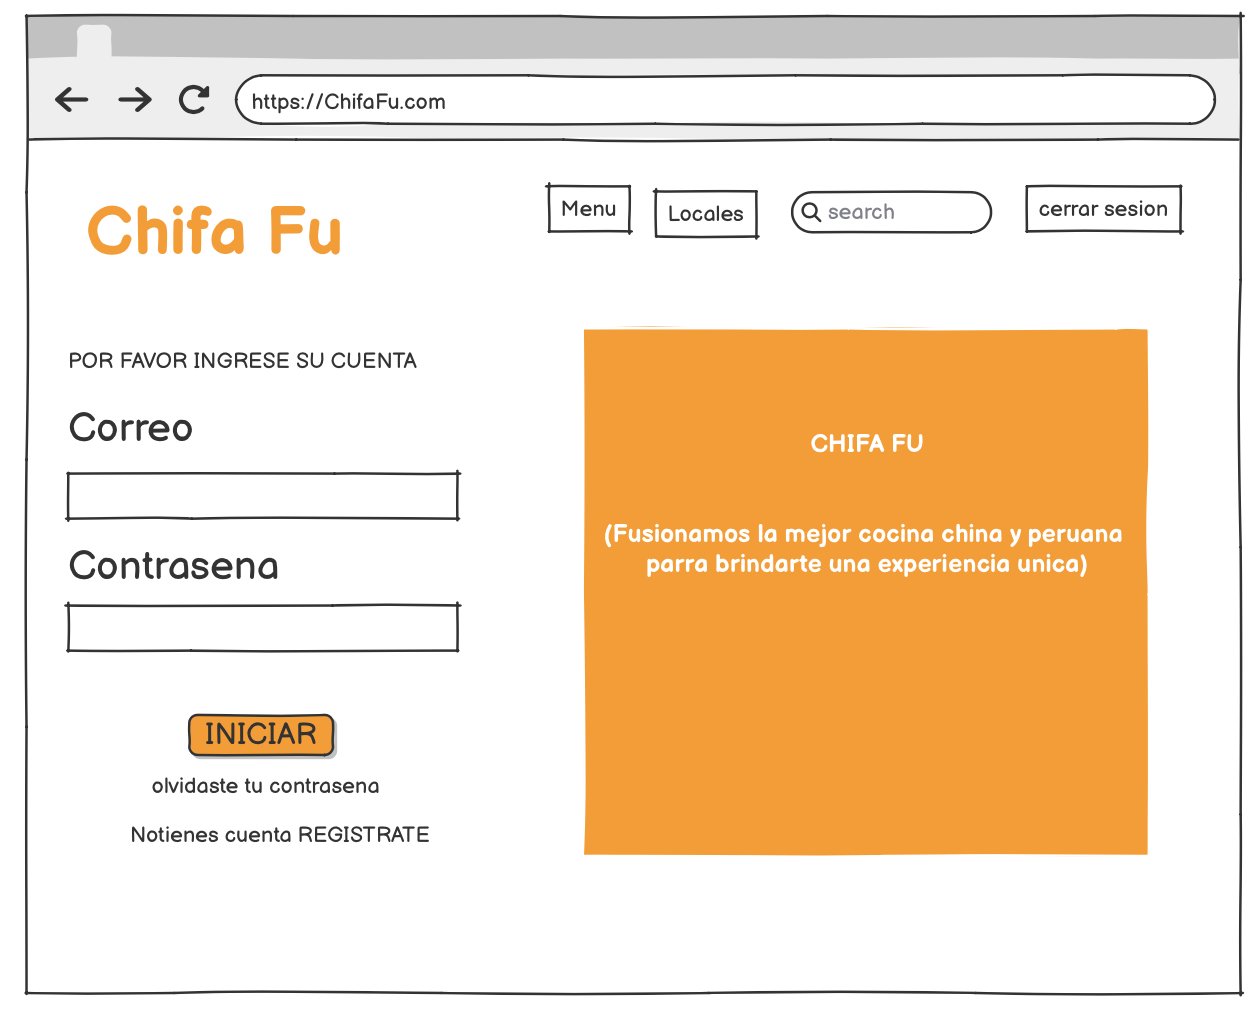
\includegraphics[width=14cm]{Solución 1/inicio.png}
        \caption{Inicio}
        \label{fig:Inicio}
    \end{figure}
    \begin{figure}[H]
        \centering
        \vspace*{1cm}
        \includegraphics[width=14cm]{Solución 1/carrito.png}
        \caption{Carrito}
        \label{fig:Carrito}
    \end{figure}
    \begin{figure}[H]
        \centering
        \vspace*{1cm}
        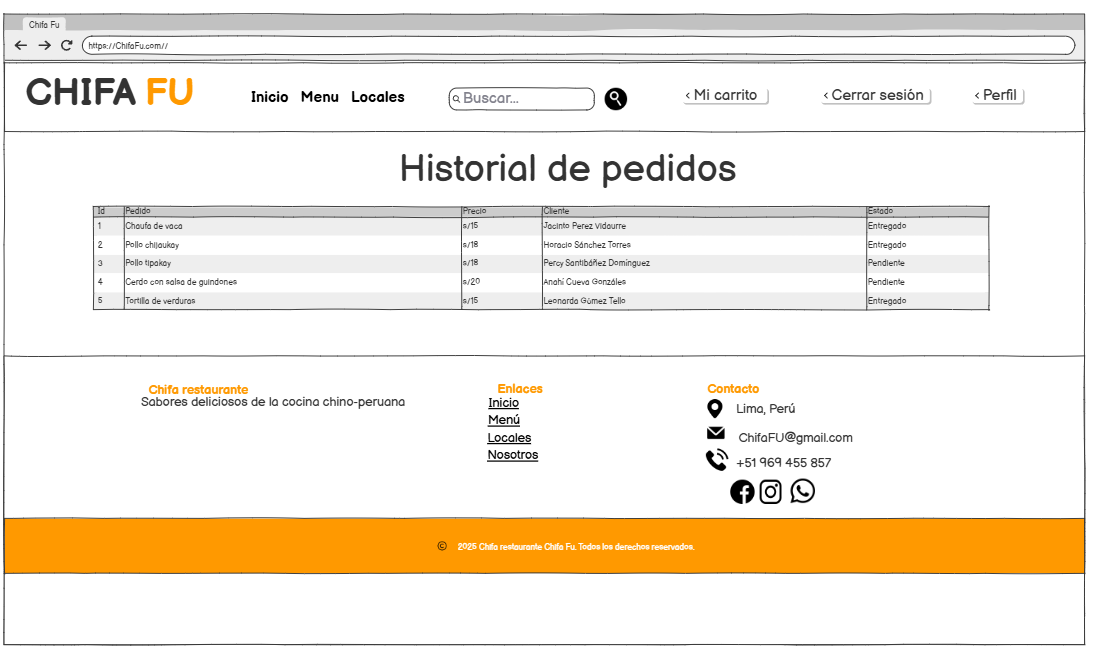
\includegraphics[width=14cm]{Solución 1/historialPedidos.png}
        \caption{Historial de pedidos}
        \label{fig:Historial-Pedidos}
    \end{figure}
    \begin{figure}[H]
        \centering
        \vspace*{1cm}
        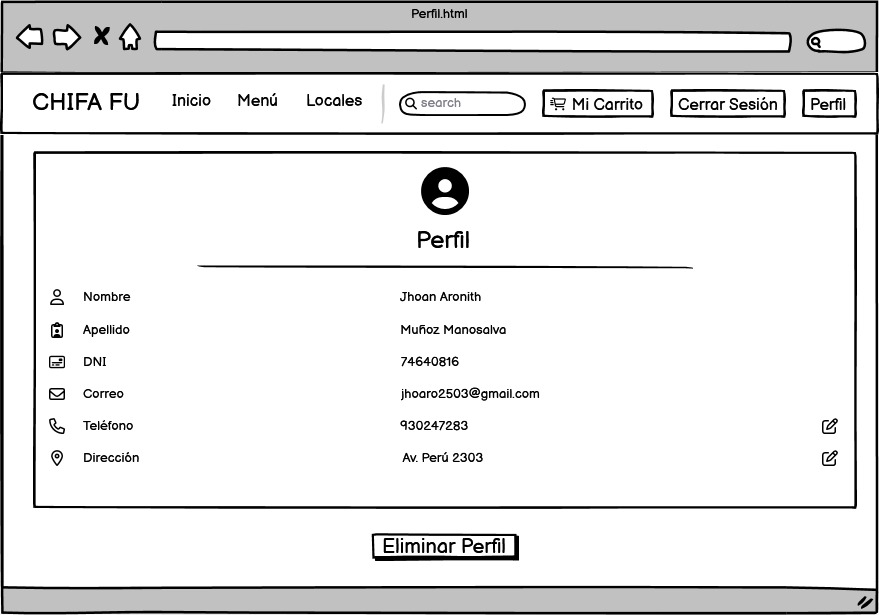
\includegraphics[width=14cm]{Solución 1/perfil.jpg}
        \caption{Perfil}
        \label{fig:Perfil}
    \end{figure}
    \begin{figure}[H]
        \centering
        \vspace*{1cm}
        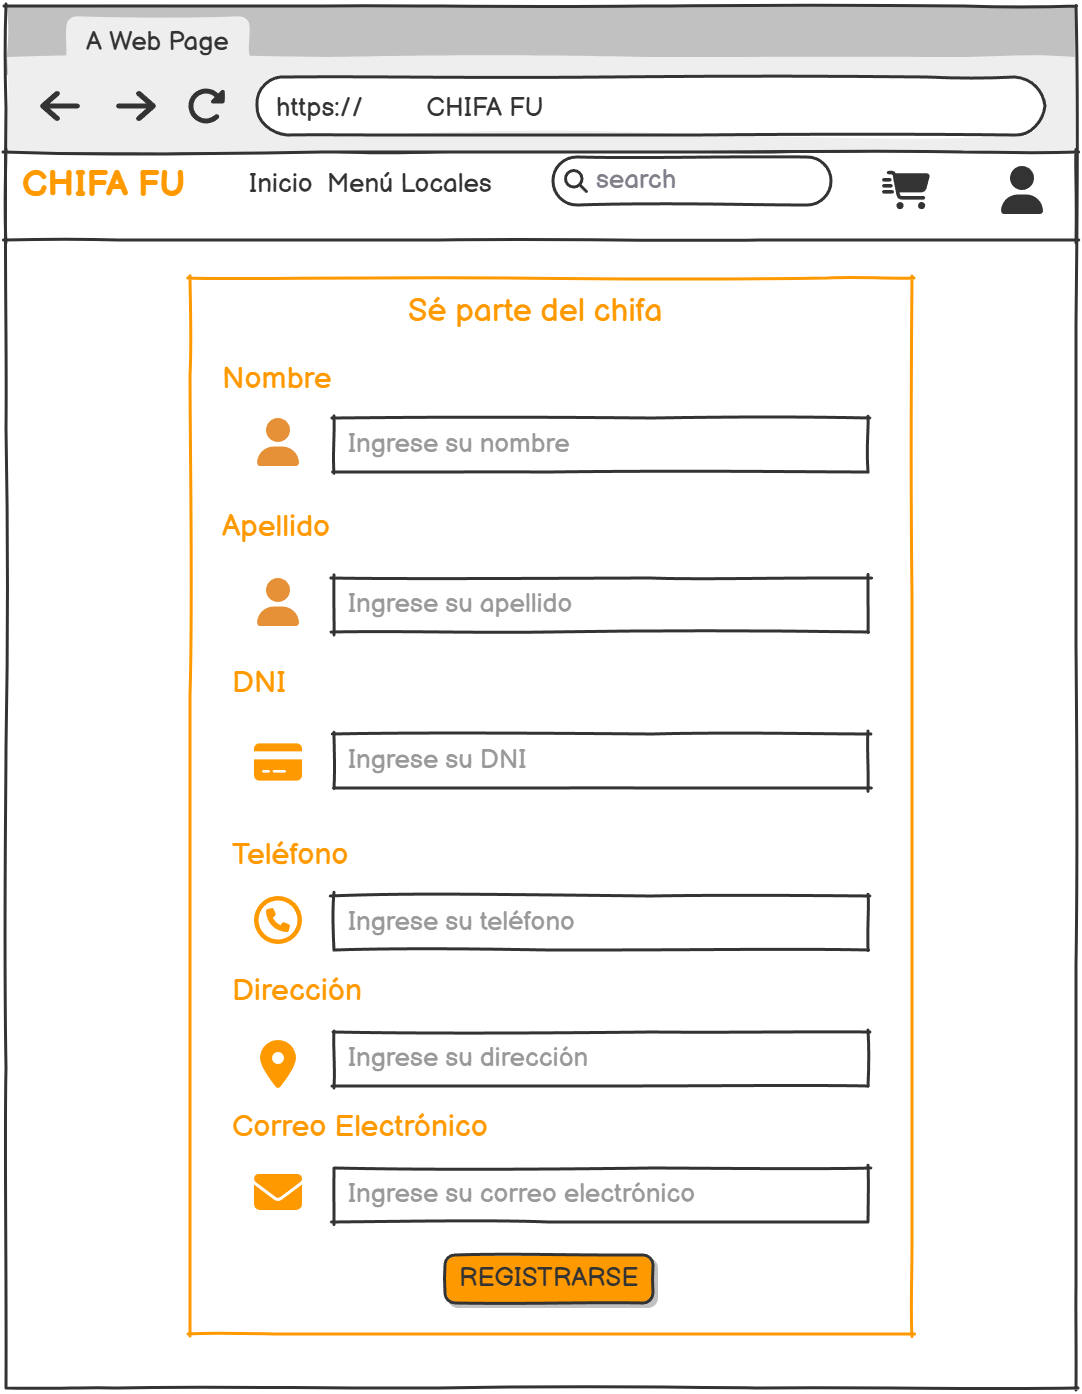
\includegraphics[width=14cm]{Solución 1/registro chifa.png}
        \caption{Registro}
        \label{fig:Registro}
    \end{figure}
    
    \subsection{Alternativa 2: Optimización de pedidos}

    \noindent Son interfaces diseñadas para hacer que el proceso de pedir sea rápido y sencillo. Incluye menú digital interactivo, carrito de compras, integración con métodos de pago, seguimiento en tiempo real e historial de pedidos.\\
    \textbf{Ventajas:}\\
    - El cliente puede personalizar su pedido fácilmente.\\
    - Pagos más ágiles gracias a la integración con billeteras digitales y tarjetas.\\
    - Mayor fidelización al permitir repetir pedidos anteriores con un clic.\\
    - Transparencia y confianza al mostrar el seguimiento del pedido en tiempo real.\\
    \textbf{Desventajas:}\\
    - Depende de una buena conexión a internet.\\
    - Algunos clientes tradicionales pueden resistirse a usar un sistema digital.\\
    - Costos de integración con pasarelas de pago externas.\\

    \begin{figure}[H]
        \centering
        \vspace*{1cm}
        \includegraphics[width=14cm]{Solución 2/carrito.png}
        \caption{Carrito}
        \label{fig:Carrito}
    \end{figure}
    \begin{figure}[H]
        \centering
        \vspace*{1cm}
        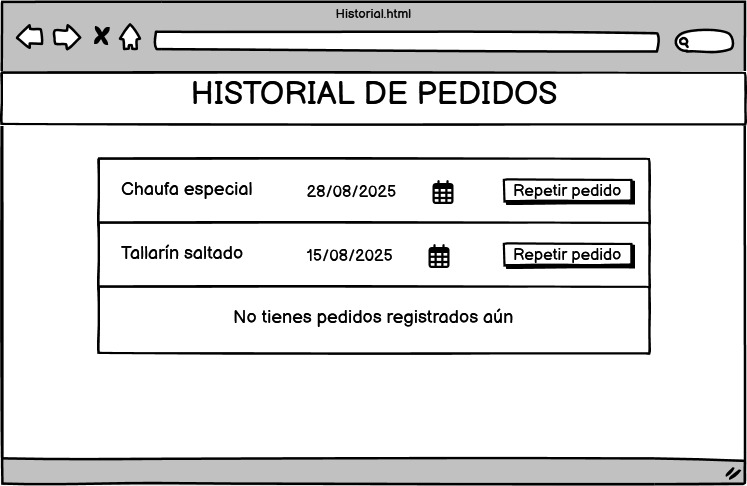
\includegraphics[width=14cm]{Solución 2/historial.jpg}
        \caption{Historial}
        \label{fig:Historial}
    \end{figure}
    \begin{figure}[H]
        \centering
        \vspace*{1cm}
        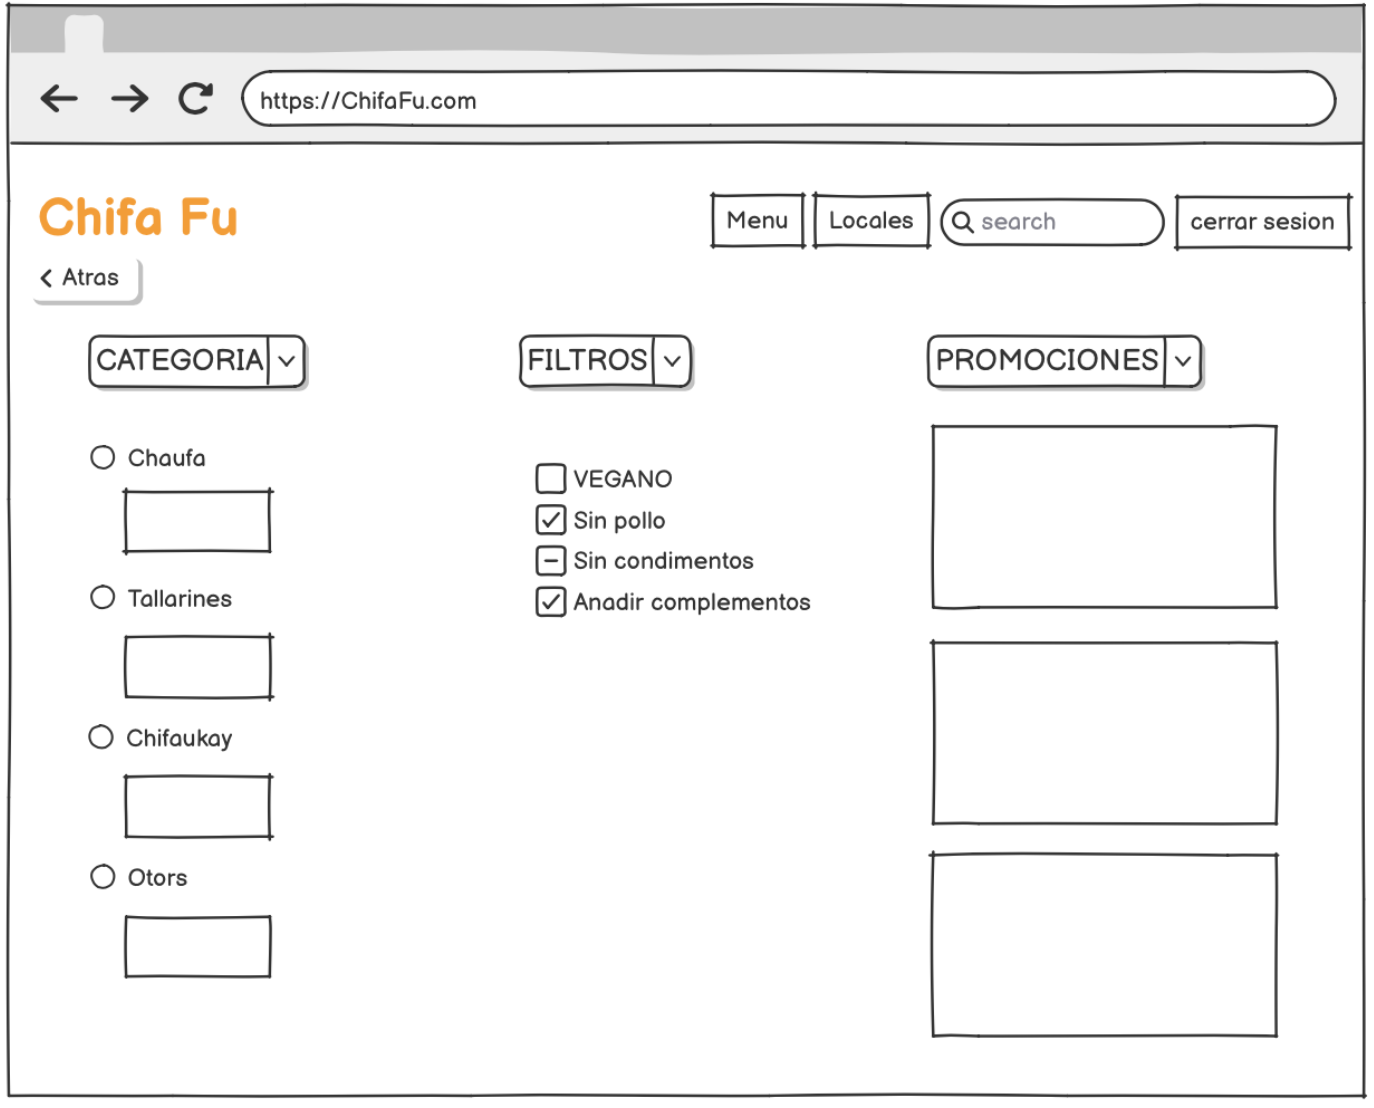
\includegraphics[width=14cm]{Solución 2/menudigital.png}
        \caption{Menu Digital}
        \label{fig:Menu-Digital}
    \end{figure}
    \begin{figure}[H]
        \centering
        \vspace*{1cm}
        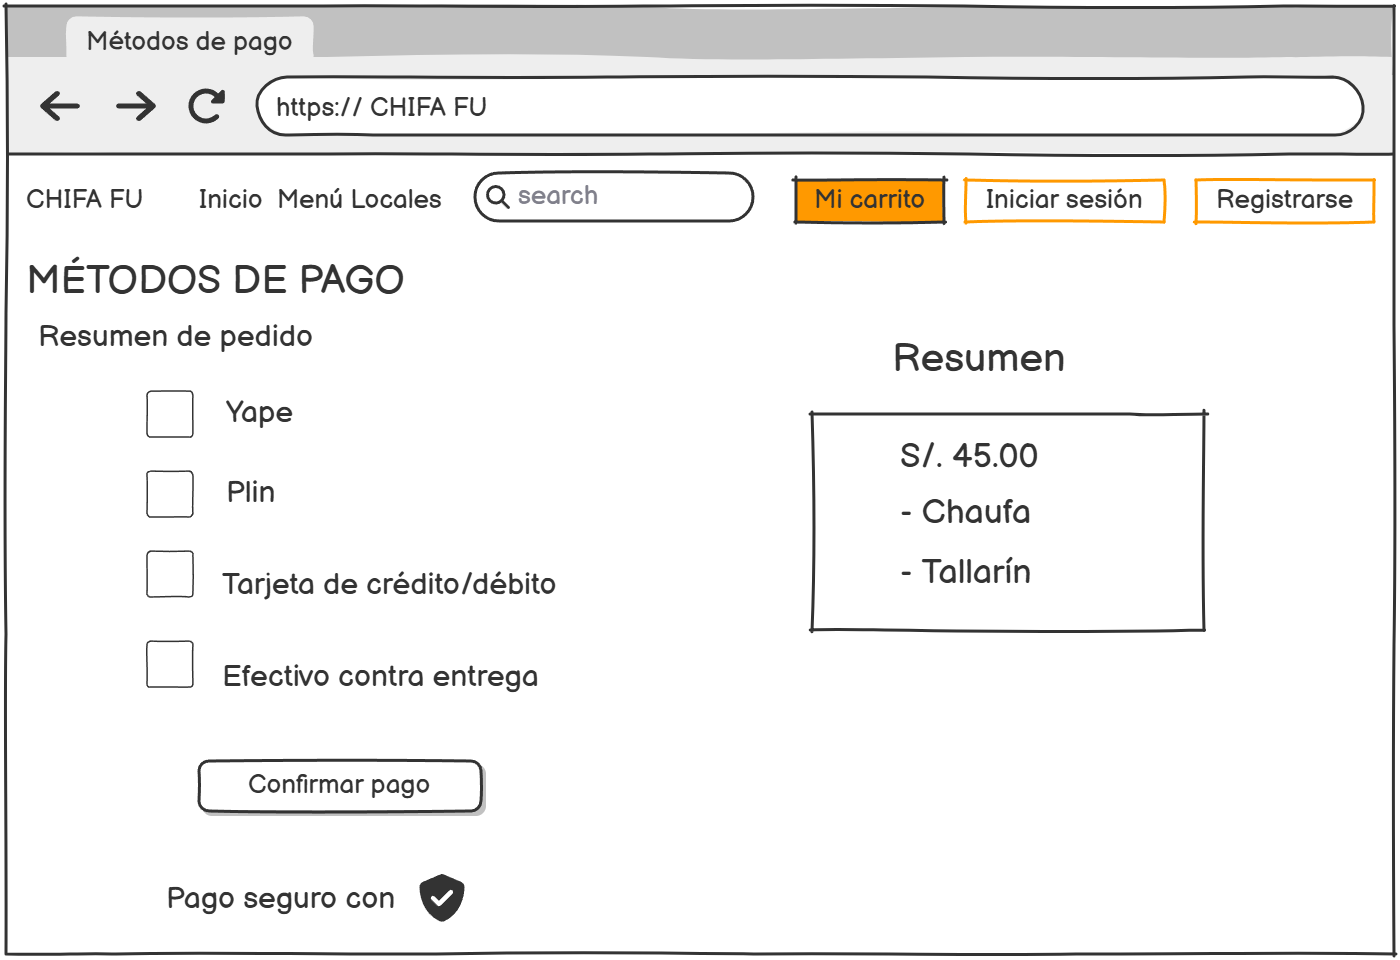
\includegraphics[width=14cm]{Solución 2/metodos de pago.png}
        \caption{metodos de pago}
        \label{fig:Metodos-de-pago}
    \end{figure}
    \begin{figure}[H]
        \centering
        \vspace*{1cm}
        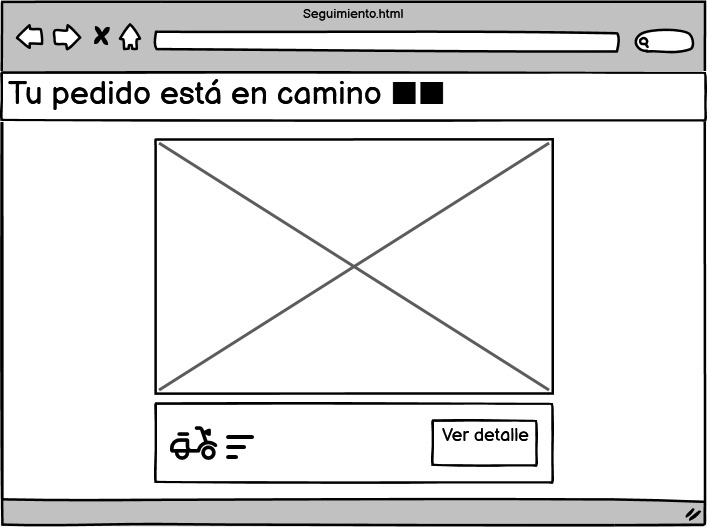
\includegraphics[width=14cm]{Solución 2/seguimiento.jpg}
        \caption{Seguimiento}
        \label{fig:Seguimiento}
    \end{figure}
    
    \subsection{Alternativa 3: Gestión de recursos humanos}

    \noindent Interfaces internas (intranet) enfocadas en el personal del chifa. Incluye un panel de empleados, gestión de turnos, control de asistencia, panel de desempeño y capacitación online.\\
    \textbf{Ventajas:}\\
    - Facilita la organización de horarios y turnos del personal.\\
    - Permite llevar un control claro de asistencia y puntualidad.\\
    - Motiva al personal con evaluaciones de desempeño basadas en reseñas reales.\\
    - Ofrece capacitación digital, lo que mejora la calidad del servicio sin necesidad de entrenamientos presenciales costosos.
    \\
    \textbf{Desventajas:}\\
    - Puede generar resistencia en trabajadores que no están familiarizados con la tecnología.\\
    - Requiere tiempo y esfuerzo inicial para digitalizar procesos de RR.HH.\\
    - Posible percepción de control excesivo (puede incomodar a algunos empleados).\\

    \begin{figure}[H]
        \centering
        \vspace*{1cm}
        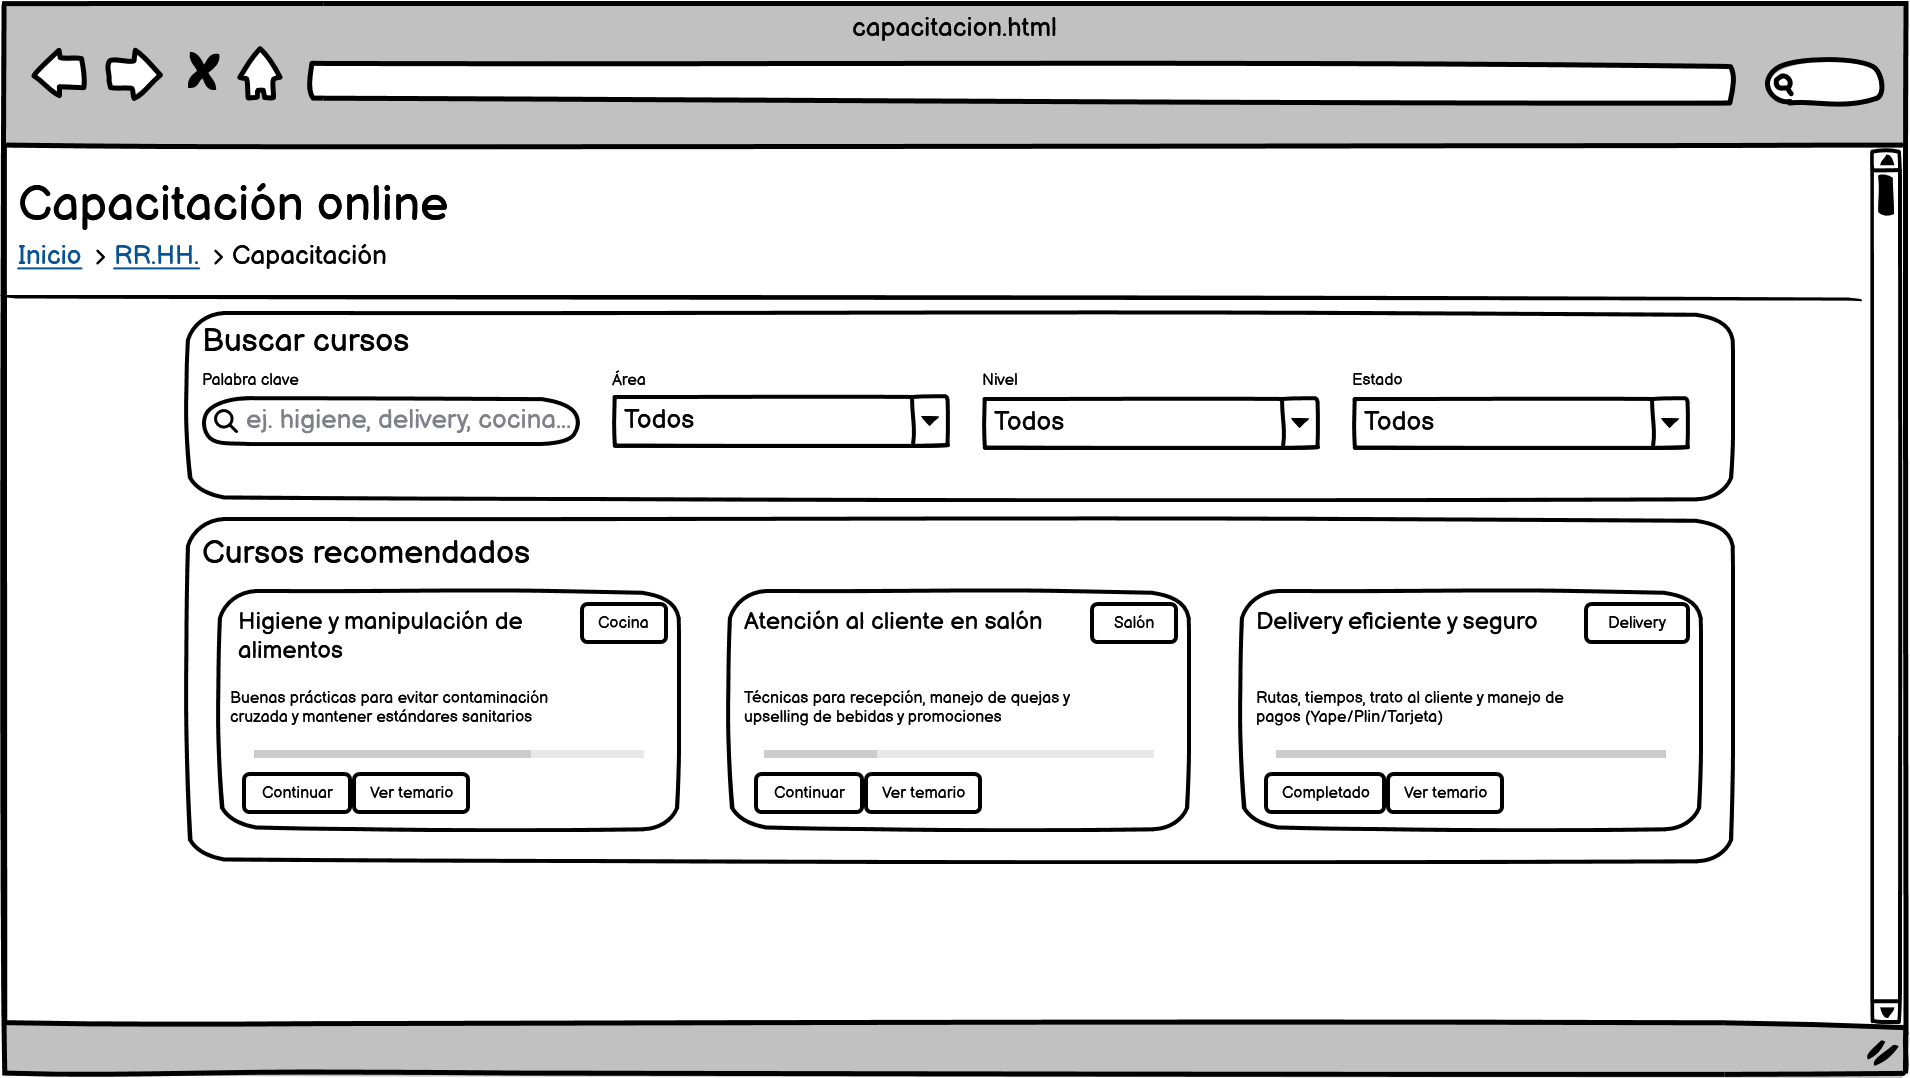
\includegraphics[width=14cm]{Solución 3/capacitacion.png}
        \caption{Capacitacion}
        \label{fig:Capacitacion}
    \end{figure}
    \begin{figure}[H]
        \centering
        \vspace*{1cm}
        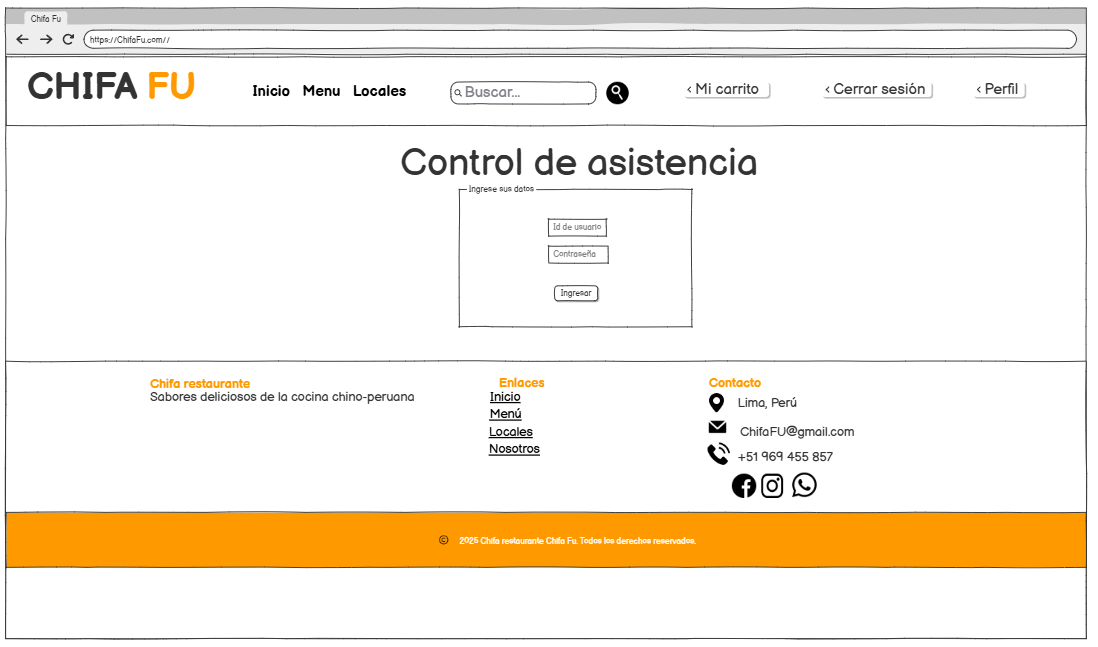
\includegraphics[width=14cm]{Solución 3/controlAsistencia.png}
        \caption{Control de asistencias}
        \label{fig:Control-de-asistencias}
    \end{figure}
    \begin{figure}[H]
        \centering
        \vspace*{1cm}
        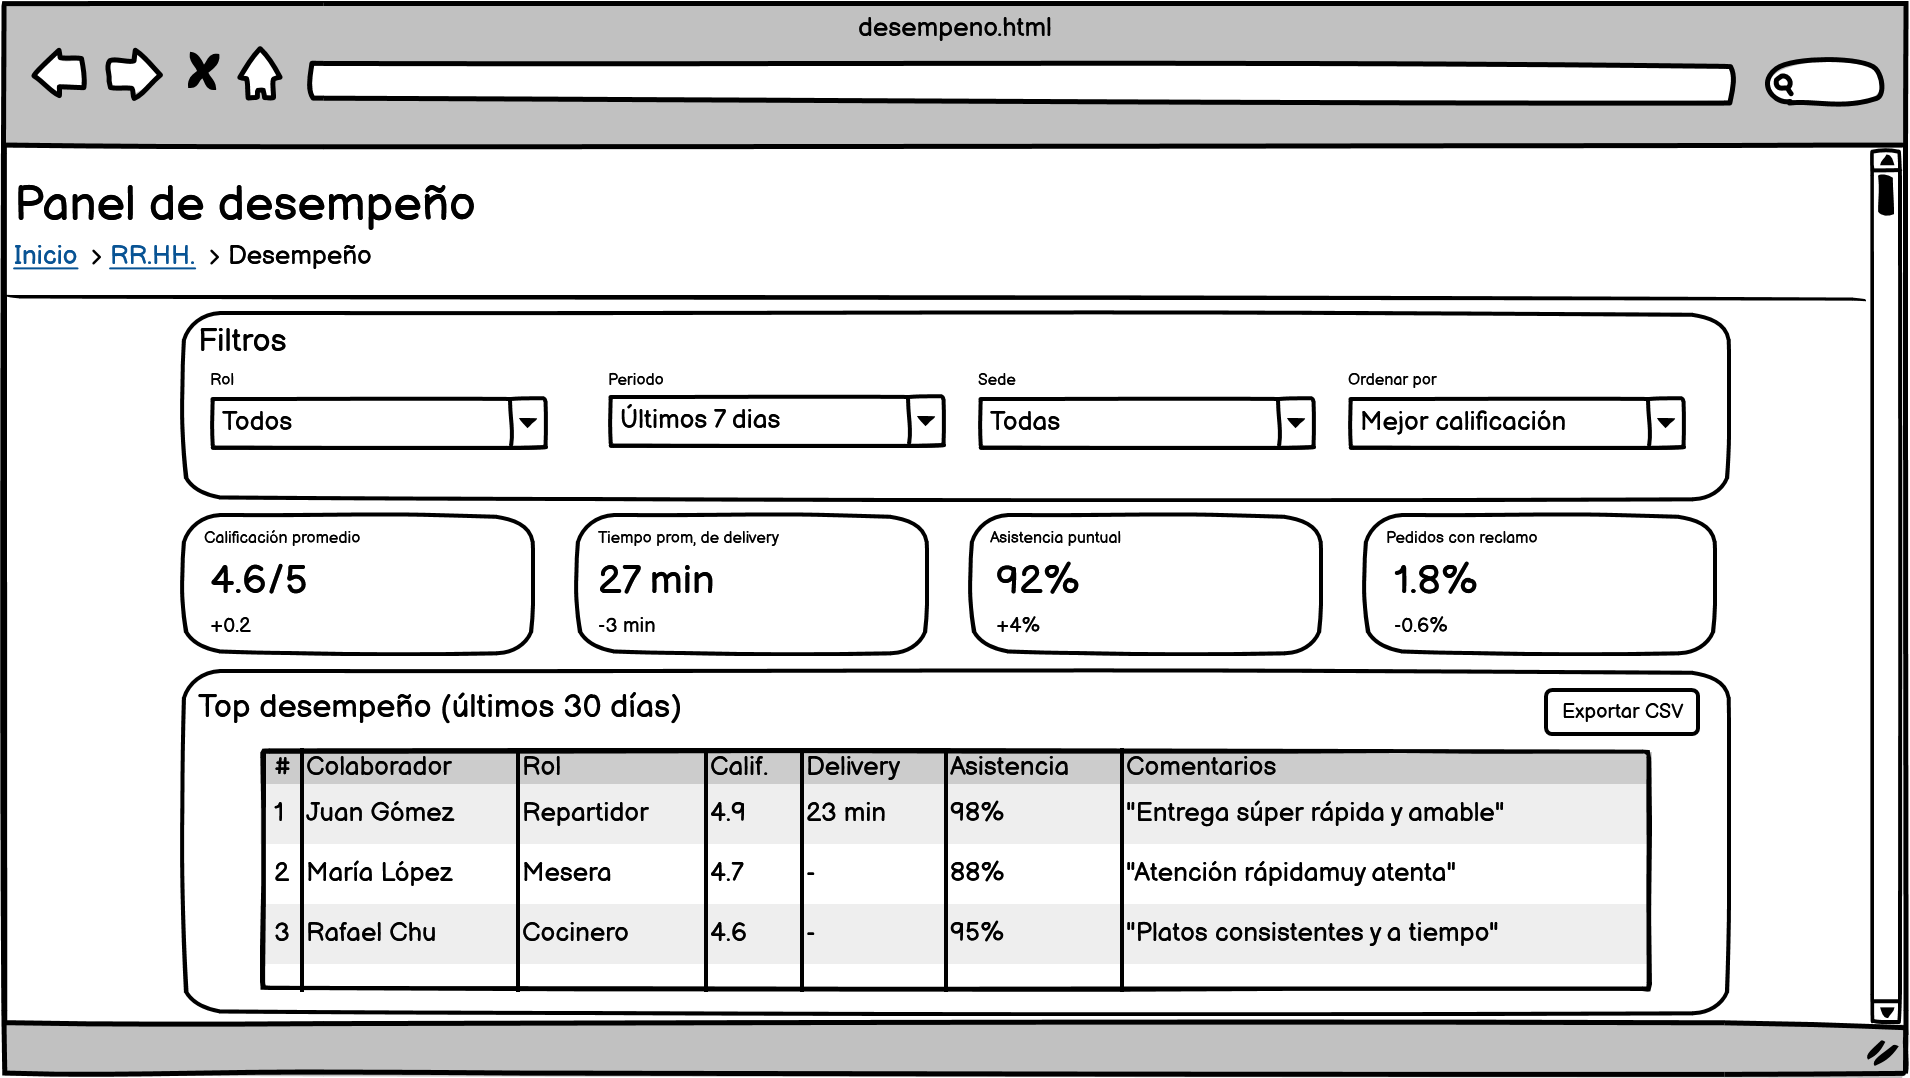
\includegraphics[width=14cm]{Solución 3/desempeno.png}
        \caption{Desempeño}
        \label{fig:Desempeno}
    \end{figure}
    \begin{figure}[H]
        \centering
        \vspace*{1cm}
        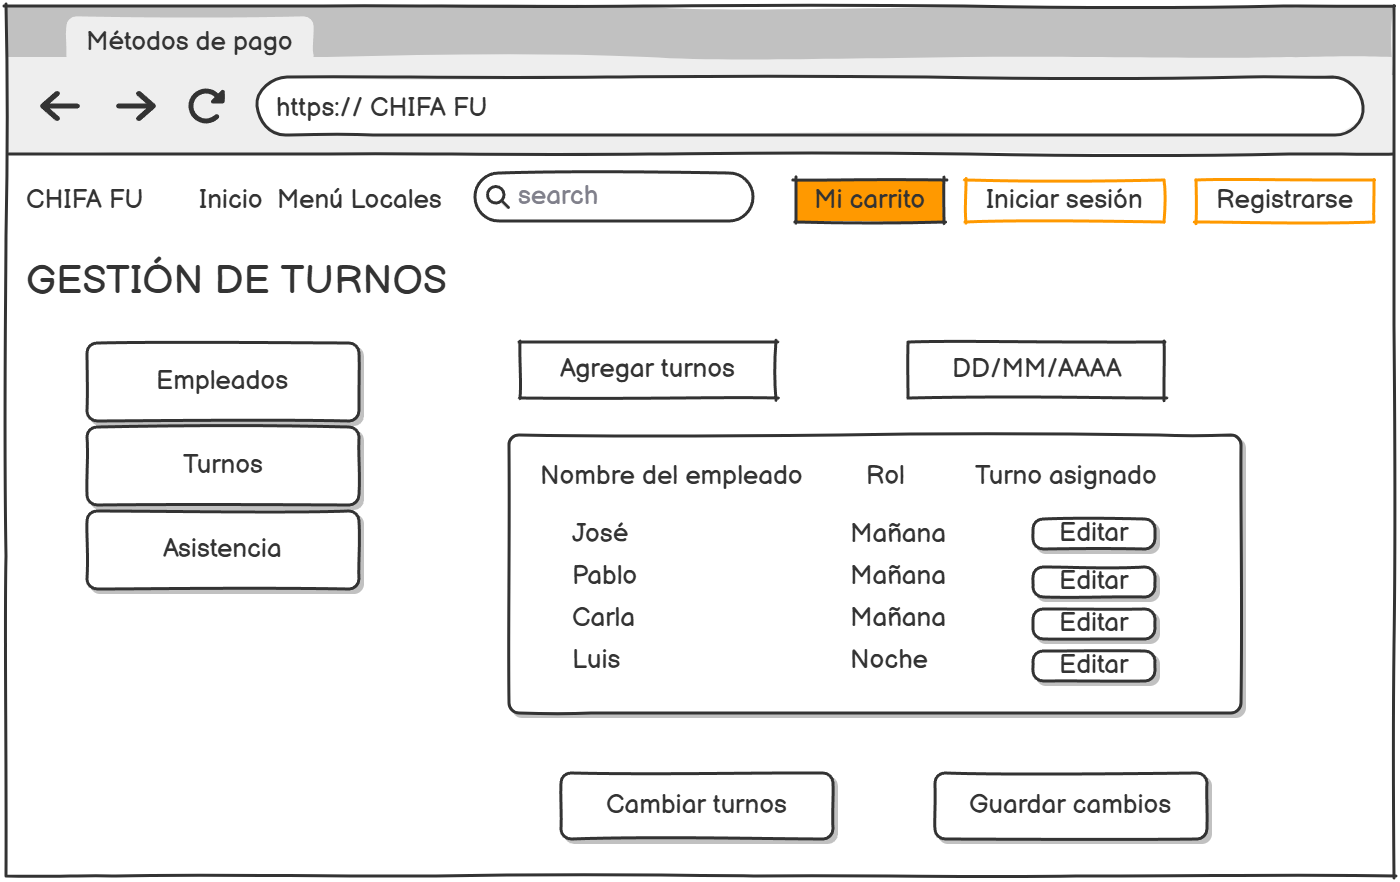
\includegraphics[width=14cm]{Solución 3/Gestion de turnos.png}
        \caption{Gestión de turnos}
        \label{fig:Gestion-de-turnos}
    \end{figure}
    \begin{figure}[H]
        \centering
        \vspace*{1cm}
        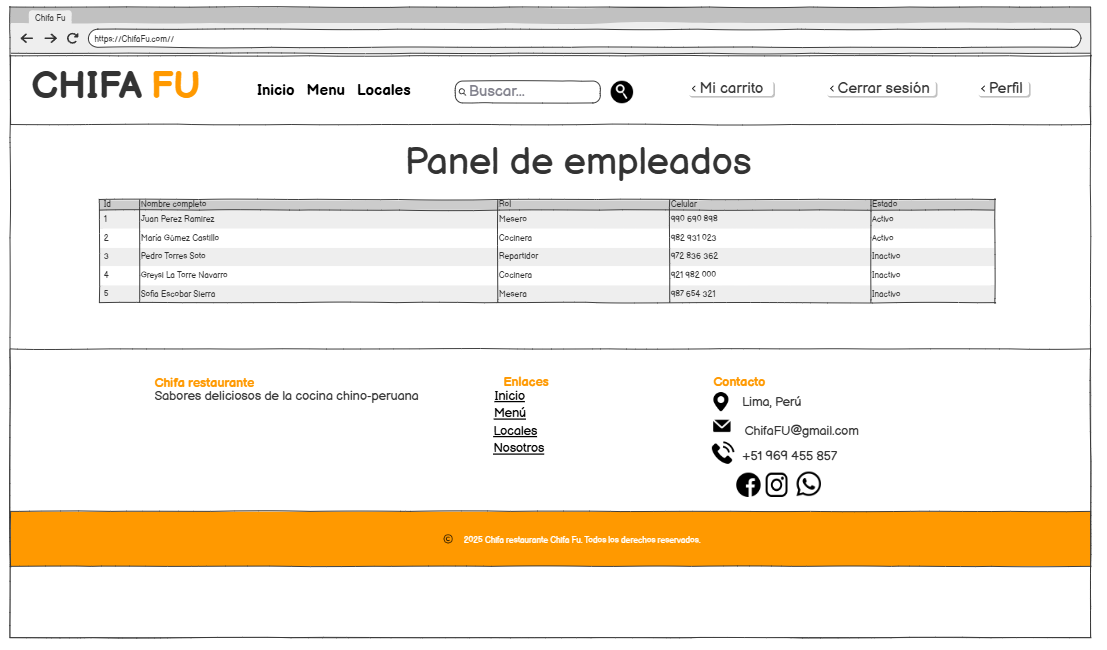
\includegraphics[width=14cm]{Solución 3/panelEmpleados.png}
        \caption{Panel de empleados}
        \label{fig:Panel-de-empleados}
    \end{figure}

\section{Diagrama Gantt}
    \noindent Aplicaremos el Diagrama de Gantt para planificar la ejecución y las etapas de nuestro proyecto.\\
    \begin{figure}[H]
        \centering
        \vspace*{1cm}
        \includegraphics[width=14cm]{img/Gantt.png}
        \caption{Diagrama Gantt}
        \label{fig:Diagrama-gantt}
    \end{figure}

\section{Project Charter}

\begin{figure}[H]
    \centering
    \includegraphics[width=\textwidth]{img/project.png}
    \caption{Project Charter}
    \label{fig:Project-Charter}
\end{figure}


\section{Estructura de desglose del trabajo (WBS)}

    \begin{figure}[H]
        \centering
        \vspace*{1cm}
        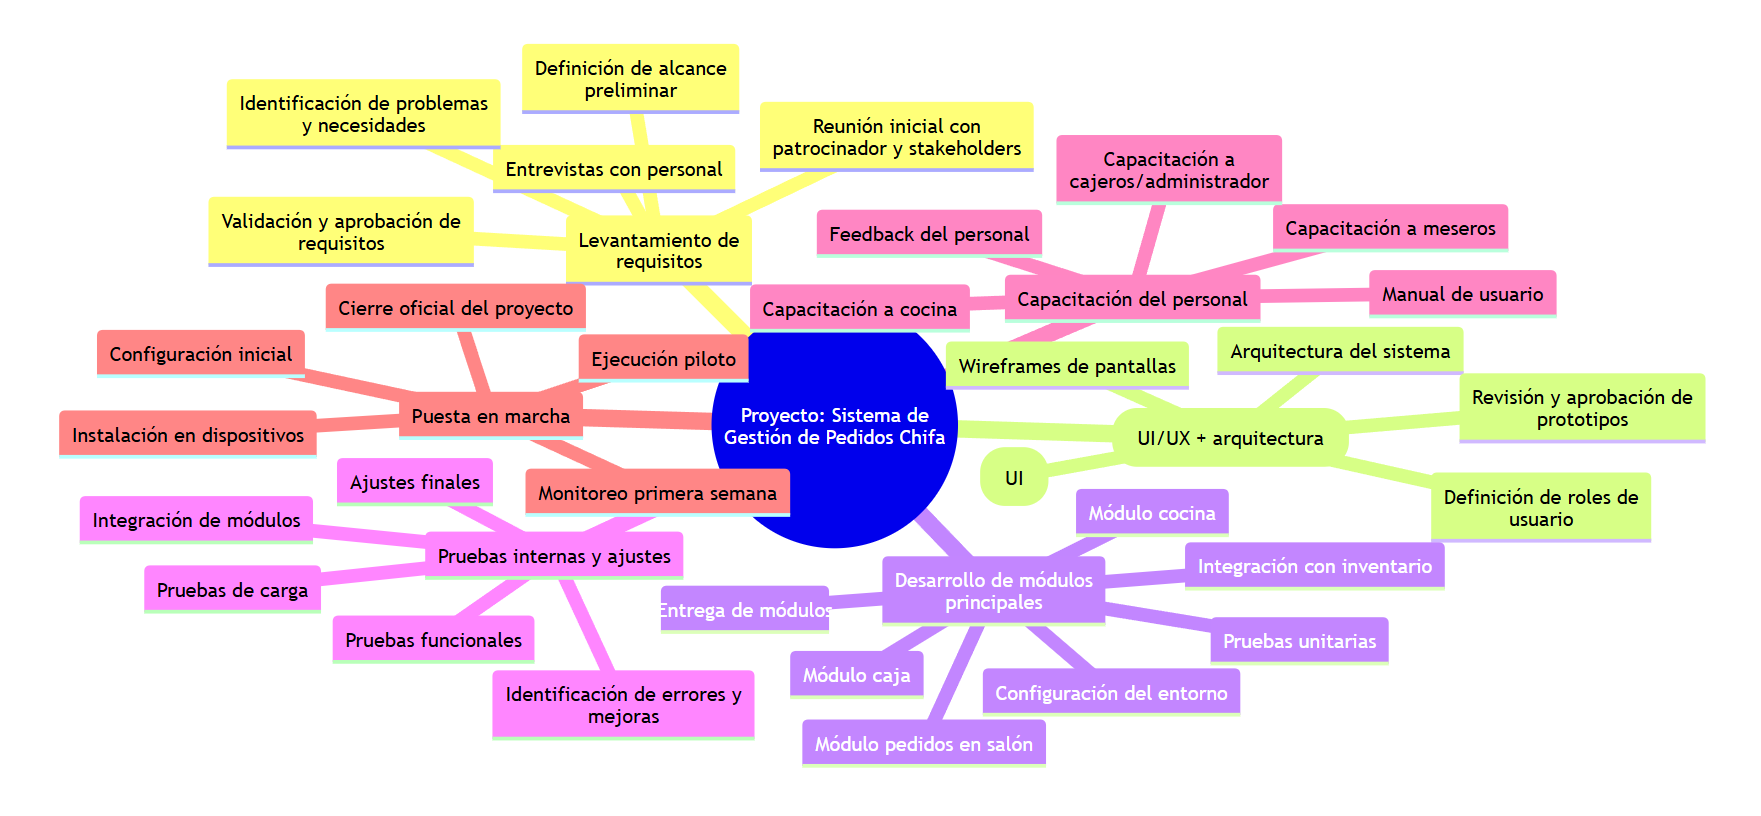
\includegraphics[width=14cm]{img/WBS.png}
        \caption{WBS}
        \label{fig:WBS}
    \end{figure}

\section{Alternativa elegida: Alternativa 1}

    \begin{figure}[H]
        \centering
        \vspace*{1cm}
        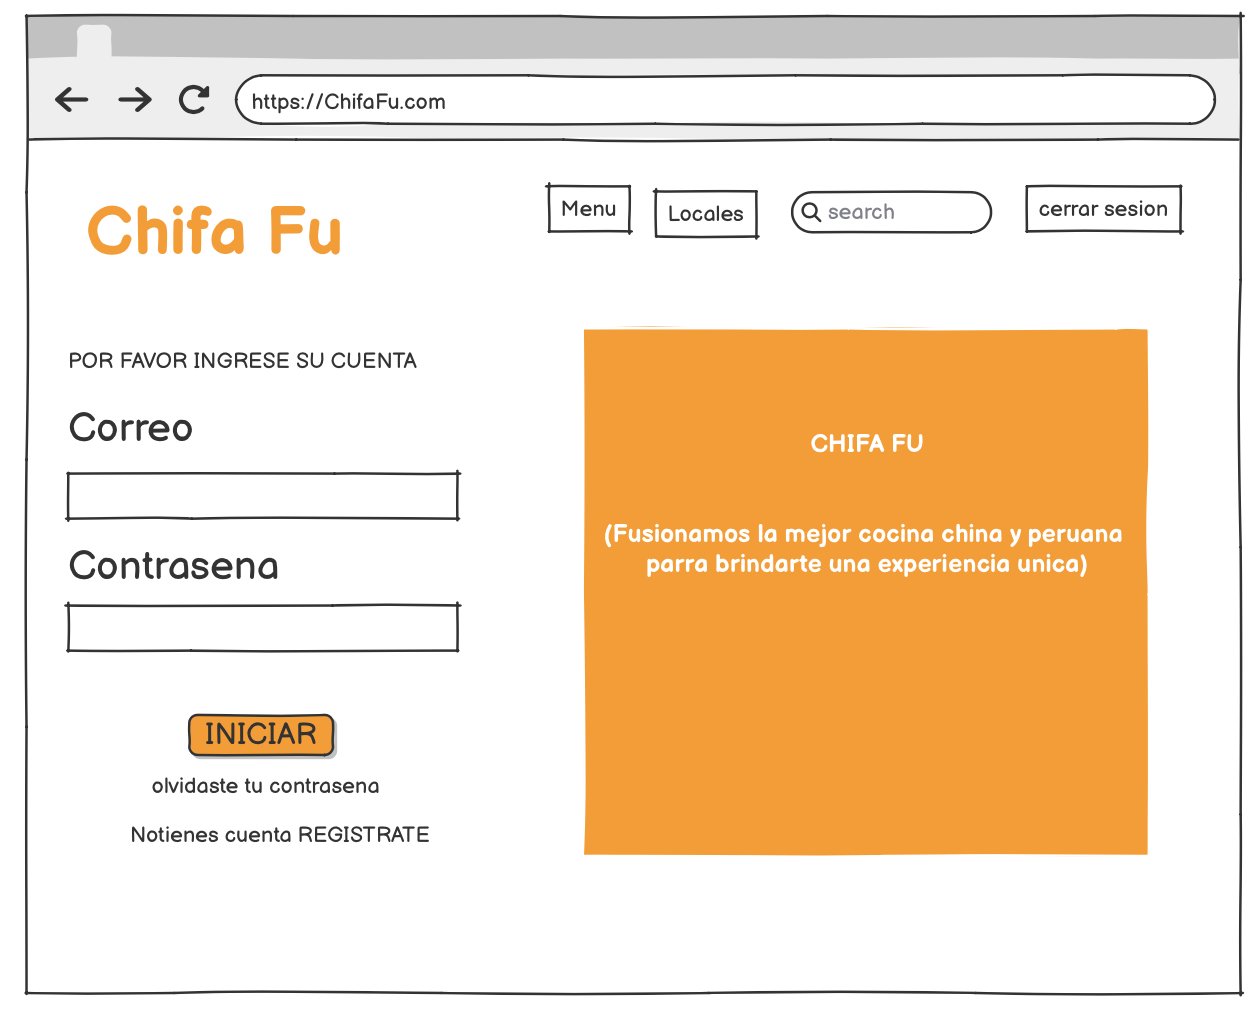
\includegraphics[width=14cm]{Solución 1/inicio.png}
        \caption{Inicio}
        \label{fig:Inicio}
    \end{figure}
    \begin{figure}[H]
        \centering
        \vspace*{1cm}
        \includegraphics[width=14cm]{Solución 1/carrito.png}
        \caption{Carrito}
        \label{fig:Carrito}
    \end{figure}
    \begin{figure}[H]
        \centering
        \vspace*{1cm}
        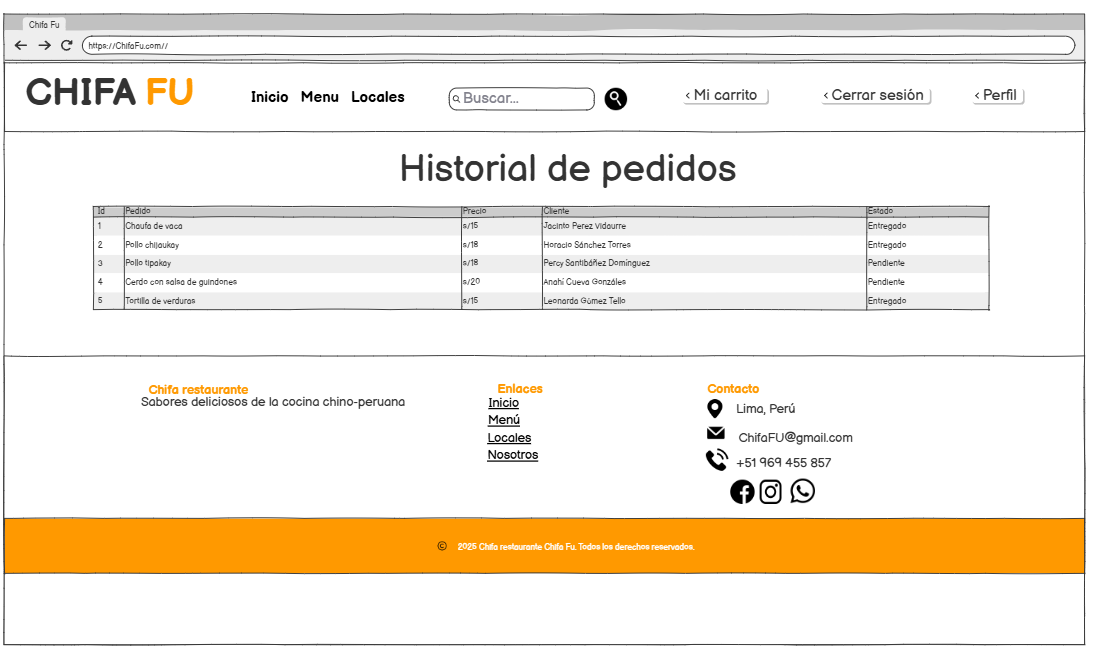
\includegraphics[width=14cm]{Solución 1/historialPedidos.png}
        \caption{Historial de pedidos}
        \label{fig:Historial-Pedidos}
    \end{figure}
    \begin{figure}[H]
        \centering
        \vspace*{1cm}
        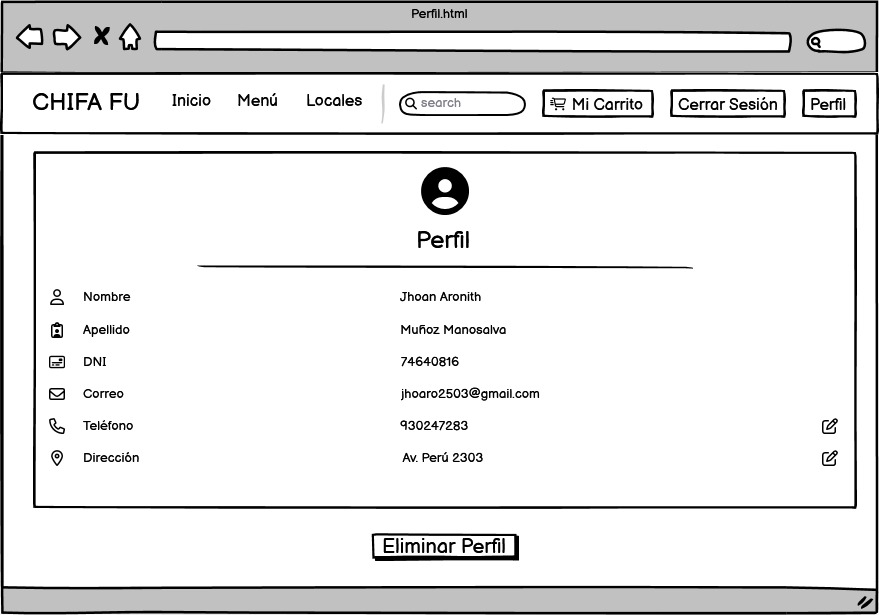
\includegraphics[width=14cm]{Solución 1/perfil.jpg}
        \caption{Perfil}
        \label{fig:Perfil}
    \end{figure}
    \begin{figure}[H]
        \centering
        \vspace*{1cm}
        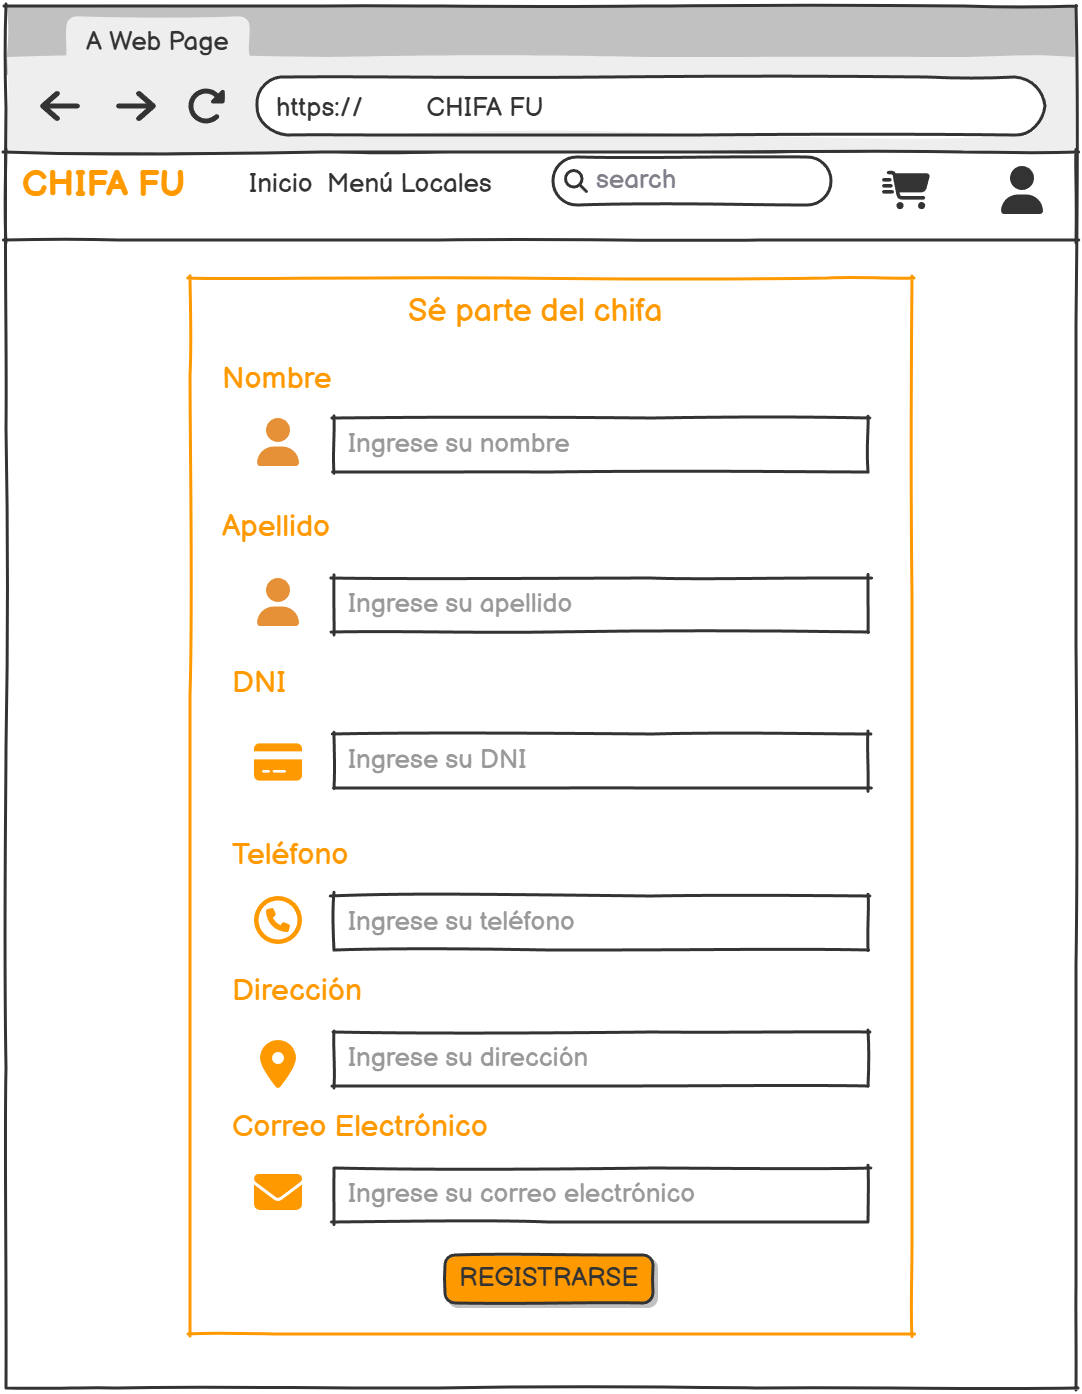
\includegraphics[width=14cm]{Solución 1/registro chifa.png}
        \caption{Registro}
        \label{fig:Registro}
    \end{figure}

    \section{Modelado BPM}
    \begin{itemize}
        
    \end{itemize}

    \section{Diagrama de procesos}
    \begin{itemize}
        
    \end{itemize}

    \begin{center}
        \textbf{Este informe fue creado utilizando \LaTeX, un sistema de composición tipográfica muy utilizado en la escritura académica y científica.}
    \end{center}

\end{doublespace}
\end{document}
